% Provenance (never printed): see sources/outline_sources.md (Year 3:
% fractionation and Rayleigh distillation in the water cycle;
% palaeothermometry; carbon and sulfur isotopes). Brief:
% sources/book5/BRIEFS.md, ch. 14. Curves from figdata/bachelor-3/
% rayleigh_distillation.py, lr04_d18o.py, carbon_mass_balance.py. Exercise
% and problem values in the Book 5 scratch calculator calc/ch14.py. Dome Ilse,
% its traverse and the marine core are invented.
\chapter{稳定同位素地球化学}\label{ch:b3:stable-isotopes}

落在东南极冰盖高处穹顶上的雪，是地球上
最轻的水之一。它的每个分子都曾以蒸气的形式离开海洋，
在向内陆输送的途中，空气以雪的形式失去了大部分水分，
其中重分子先落下。到达时剩下的水量，取决于损失了多少，而这又
取决于空气变得有多冷。因此，一柱冰是一支温度计，一个
方解石壳是另一支，石灰岩中的碳则是一本账，记录生物圈
埋藏了什么。本章推导这些记录背后的规律，
并加以解读。

\begin{recall}
$\delta$ 值、分馏系数 $\alpha$ 以及平衡与
动力学同位素效应见化学系列的大学分册。
参考标准 VSMOW 与 VPDB，以及大气降水线，见
本科二年级分册中关于同位素地球化学的一章；微量元素的瑞利
分馏定律见其中关于岩浆分异的一章；气候替代指标、冰量效应
与 Mg/Ca 温度计见其中关于气候档案与替代指标的一章；
古新世–始新世极热事件见其中关于
地质历史时期气候的一章；大氧化事件见其中关于
前寒武纪地球的一章。
光合作用与细菌硫酸盐还原见生物学书籍。
\end{recall}

\section{两相之间的分馏}\label{sec:b3:stable-isotopes:fractionation}

对于处于同位素平衡的两相 A 和 B，$\alpha_{A-B} = R_A/R_B =
(1000 + \delta_A)/(1000 + \delta_B)$，其中 $R$ 为重同位素与轻同位素的比值。
水蒸气与液态水之间，氧-18 的 $\alpha = 1.0098$，
在 \qty{20}{\celsius} 时，氘为 $1.084$；在 \qty{0}{\celsius} 时，二者分别为 $1.0117$ 和 $1.111$；
冰与水之间，在 \qty{0}{\celsius} 时分别为 $1.0035$ 和 $1.0208$。
较重的相总是凝结程度更高的那一相，分馏程度
随温度降低而增大。
% ledger: kc98:alpha, kc98:standards

\begin{definition}[同位素差值]\label{def:b3:stable-isotopes:big-delta}
称两相之间的\emph{同位素差值}\index{同位素差值（大写 Delta）}
为 $\Delta_{A-B} = \delta_A - \delta_B$，单位为 ‰。
\end{definition}

\begin{proposition}[同位素差值与分馏系数]
\label{prop:b3:stable-isotopes:big-delta}
当 $\alpha$ 接近 1 且 $\delta$ 值较小时，
\[
\Delta_{A-B} \approx 1000\ln\alpha_{A-B} \approx 1000(\alpha_{A-B} - 1).
\]
\end{proposition}

\begin{proof}
$1000\ln\alpha = 1000\ln(1 + \delta_A/1000) - 1000\ln(1 + \delta_B/1000)$，且
$1000\ln(1 + x/1000) = x - x^2/2000 + \dots$，因此 $1000\ln\alpha = \delta_A -
\delta_B - (\delta_A^2 - \delta_B^2)/2000 + \dots$。最后，$\ln\alpha \approx
\alpha - 1$（当 $\alpha$ 接近 1 时）。
\end{proof}

误差为 $(\delta_A^2 - \delta_B^2)/2000$：在海水的数值下，
只有千分之几；而在海水与极地冰的
轻雪之间，误差接近 1‰。
理论与温度相关联的量是 $1000\ln\alpha$：它
在高温下近似按 $1/T^2$ 变化，在低温下按 $1/T$ 变化，
因此标定式通常以这一形式写出。例如对冰与蒸气，
\[
\ln\alpha^{18}_{\mathrm{ice-v}} = \frac{11.839}{T} - 0.028224, \qquad
\ln\alpha^{\mathrm D}_{\mathrm{ice-v}} = \frac{16288}{T^2} - 0.0934,
\]
其中 $T$ 以开尔文为单位。
% ledger: gkinis14:alpha-ice, kc98:standards

\begin{definition}[质量相关分馏与非质量相关分馏]\label{def:b3:stable-isotopes:mif}
具有三种或以上同位素的元素，若其同位素比值的分馏量之比
与由质量决定的质量差之比一致，则称其发生\emph{质量相关分馏}\index{质量相关分馏}；
否则称其发生\emph{非质量相关分馏}\index{非质量相关分馏}，
以偏离质量相关分馏线的程度来度量，
例如对硫可取
$\Delta^{33}\mathrm S = \delta^{33}\mathrm S
- 0.515\,\delta^{34}\mathrm S$。
\end{definition}

对于氧，$^{17}\mathrm O/^{16}\mathrm O$ 的分馏量约为
$^{18}\mathrm O/^{16}\mathrm O$ 的 0.52 倍，接近质量差之比 1 比 2；
对于硫，$\delta^{33}\mathrm S = 0.515\,\delta^{34}\mathrm S$。
\omterm{def:b3:stable-isotopes:mif}{非质量相关分馏}很少见：它见于陨石、平流层臭氧以及
太古宙的硫中。
% ledger: white13c9:mdf, white13c9:s-mif

\section{水循环中的瑞利蒸馏}\label{sec:b3:stable-isotopes:rayleigh}

气团冷却时会形成云滴或雪晶，它们落下并
离开系统。每份凝结物都比蒸气更富集重同位素，因此
剩余蒸气越来越轻，而与之处于平衡的下一份凝结物
同样更轻。

\begin{proposition}[瑞利蒸馏]\label{prop:b3:stable-isotopes:rayleigh-distillation}
设蒸气储库通过凝结物失去水分，每份凝结物一经形成便被移出，
且其与蒸气处于平衡。若 $f$ 为剩余蒸气的比例，
$\alpha$ 为凝结物与蒸气之间的分馏系数，则
蒸气的比值满足 $\mathrm d\ln R_v = (\alpha - 1)\,\mathrm d\ln f$。
若 $\alpha$ 为常数，则此即\emph{瑞利
蒸馏}\index{瑞利蒸馏}：
\[
\frac{R_v}{R_{v,0}} = f^{\,\alpha - 1}, \qquad
\delta_v = (1000 + \delta_{v,0})\,f^{\,\alpha - 1} - 1000,
\]
且在 $f$ 时形成的凝结物，其 $\delta_c = \alpha(1000 + \delta_v) - 1000$。
\end{proposition}

\begin{proof}
设 $N$ 为蒸气分子数（几乎全为轻分子），$N R_v$
为重分子数。移去 $\mathrm dN < 0$ 个凝结物分子，
即移去 $\alpha R_v\,\mathrm dN$ 个重分子：$\mathrm d(NR_v) = \alpha
R_v\,\mathrm dN$。由此 $N\,\mathrm dR_v = (\alpha - 1)R_v\,\mathrm dN$，
此即取 $f = N/N_0$ 时的微分定律。若 $\alpha$ 为常数，
积分即得幂律。
\end{proof}

当 $\alpha$ 依赖于温度时，有 $\ln(R_v/R_{v,0}) = \int(\alpha - 1)\,
\mathrm d\ln f$（沿路径积分）。对于在恒压下冷却的气团，
其所能容纳的蒸气量由饱和蒸气压决定，故 $f =
e_s(T)/e_s(T_0)$，其中饱和蒸气压在 \qty{0}{\celsius} 以下
由冰的升华曲线给出。下图对一个蒸气起始于 \qty{0}{\celsius} 的气团，
积分该定律，假定其 $\delta^{18}\mathrm O = -20$，
$\delta\mathrm D = \qty{-150}{\permil}$。海洋上方的实际蒸气比与海水达到平衡时所应有的更轻，
就氧-18 而言约为 $-13$，而非 \qty{-9}{\permil}，
这是因为蒸发部分地属于动力学过程。
% ledger: iapws:melt-subl, gkinis14:alpha-ice, white13c9:rayleigh

\begin{definition}[氘盈余]\label{def:b3:stable-isotopes:d-excess}
水样的\emph{氘盈余}\index{氘盈余}为 $d =
\delta\mathrm D - 8\,\delta^{18}\mathrm O$，单位为‰。
\end{definition}

北半球大陆的降水落在直线
$\delta\mathrm D = 8.0\,\delta^{18}\mathrm O + 10$ 上，其\omterm{def:b3:stable-isotopes:d-excess}{氘盈余}约为 \qty{10}{\permil}。
斜率 8 接近两种同位素在凝结过程中平衡分馏之比。
盈余为 10 而非 0，记录了海洋上的动力学蒸发。
样品的盈余则
反映其水体蒸发偏离平衡的程度。
% ledger: dansgaard64:effects, kc98:mwl

\begin{omfigure}
\begin{tikzpicture}
\begin{groupplot}[group style={group size=2 by 1, horizontal sep=1.6cm},
  omrecord, width=0.47\linewidth, height=0.42\linewidth, title style={font=\small},
  tick label style={font=\scriptsize}, label style={font=\small},
  legend style={font=\scriptsize, legend cell align=left}]
\nextgroupplot[title={(a) 沿冷却路径},
  xlabel={凝结温度（\unit{\celsius}）}, ylabel={$\delta^{18}\mathrm O$（\unit{\permil}）},
  xmin=-55, xmax=0, ymin=-130, ymax=0, x dir=reverse,
  legend style={at={(0.03,0.03)}, anchor=south west}]
% computed in figdata/bachelor-3/rayleigh_distillation.py
\addplot[omDef, thick, densely dashed] table[x=t, y=d18v] {figdata/out/bachelor-3-rayleigh_distillation-curve.dat};
\addlegendentry{蒸气}
\addplot[omDef, thick] table[x=t, y=d18s] {figdata/out/bachelor-3-rayleigh_distillation-curve.dat};
\addlegendentry{雪}
\addplot[red!70!black, only marks, mark=*, mark size=1.6pt] table[x=t, y=d18s] {figdata/out/bachelor-3-rayleigh_distillation-stations.dat};
\addlegendentry{站点}
\nextgroupplot[title={(b) $\delta\mathrm D$--$\delta^{18}\mathrm O$ 图上的雪},
  xlabel={$\delta^{18}\mathrm O$（\unit{\permil}）}, ylabel={$\delta\mathrm D$（\unit{\permil}）},
  xmin=-110, xmax=0, ymin=-700, ymax=0,
  legend style={at={(0.97,0.03)}, anchor=south east}]
\addplot[omDef, thick] table[x=d18s, y=dDs] {figdata/out/bachelor-3-rayleigh_distillation-curve.dat};
\addlegendentry{模型雪}
\addplot[black, densely dotted, domain=-110:0, samples=2] {8*x + 10};
\addlegendentry{$\delta\mathrm D = 8\,\delta^{18}\mathrm O + 10$}
\addplot[red!70!black, only marks, mark=*, mark size=1.6pt, forget plot] table[x=d18s, y=dDs] {figdata/out/bachelor-3-rayleigh_distillation-stations.dat};
\end{groupplot}
\end{tikzpicture}

\par\smallskip{\small 对恒压冷却气团作\omterm{prop:b3:stable-isotopes:rayleigh-distillation}{瑞利蒸馏}，起始蒸气温度为 \qty{0}{\celsius}，
所用冰–蒸气分馏系数与剩余蒸气比例均由冰的升华曲线读出。（a）蒸气（虚线）
与雪（实线）的同位素值越来越轻，且下降越来越快；圆点为周末问题中的三个站点。
（b）模型雪在氧-18 约降至 \qty{-30}{\permil}
之前紧贴大气降水线，
此后升至其上方。
}\label{fig:b3:stable-isotopes:rayleigh}
\end{omfigure}
% ledger: kc98:mwl


\begin{definition}[温度效应、降水量效应与大陆效应]\label{def:b3:stable-isotopes:effects}
\emph{温度效应}\index{温度效应（同位素）}是指降水的
$\delta^{18}\mathrm O$ 与 $\delta\mathrm D$ 随当地气温降低而减小；
在热带地区，二者随降雨量增加而减小，称为\emph{降水量效应}\index{降水量效应}；
而\emph{大陆效应}\index{大陆效应}是指二者在
给定温度下向内陆方向减小，
亦即温度保持不变。
\end{definition}

三者均可视为从地面看到的\omterm{prop:b3:stable-isotopes:rayleigh-distillation}{瑞利蒸馏}。在高纬度地区，
\omterm{def:b3:stable-isotopes:effects}{温度效应}占主导：格陵兰与北大西洋站点的年均值满足
$\delta^{18}\mathrm O = 0.69\,t - 13.6$ 与 $\delta\mathrm D =
5.6\,t - 100$（单位为‰，$t$ 为年平均地表温度，单位为 \unit{\celsius}）。在热带地区则
\omterm{def:b3:stable-isotopes:effects}{降水量效应}占主导：在某一海洋岛屿上，
月降水量每增加 \qty{100}{mm}，降水中的氧-18 约减少 \qty{1.6}{\permil}。
上图中的简单模型给出的斜率更陡，
约为每一度凝结温度 \qty{1.6}{\permil}。
两种斜率不能直接比较：冰盖表面比形成雪的空气更冷，
且模型忽略了气团的混合与雪形成时的动力学效应，因此
相对于地表温度的斜率，
是标定得到的，而非计算得到的。
% ledger: dansgaard64:effects

\section{古温度测定}\label{sec:b3:stable-isotopes:palaeothermometry}

\begin{definition}[古温度测定、古温度方程]
\label{def:b3:stable-isotopes:palaeothermometry}
\emph{古温度测定}\index{古温度测定}是利用当时形成的材料成分，
测定过去的温度。
\emph{古温度方程}\index{古温度方程}是一种经标定的关系，
将矿物的形成温度与其生长所用水体之间的分馏
联系起来。
\end{definition}

对于从水中缓慢沉淀的方解石，一种标定式给出：
\[
1000\ln\alpha_{\mathrm{calcite-water}} = 18.03\,\frac{10^3}{T} - 32.42,
\]
两者的 $\delta$ 值均取 VSMOW 标度。碳酸盐则以 VPDB 标度报告，
换算式为 $\delta^{18}\mathrm O_{\mathrm{VPDB}} =
0.97001\,\delta^{18}\mathrm O_{\mathrm{VSMOW}} - 29.99$。在 \qty{5}{\celsius} 附近，
每升温一度，分馏值约下降 \qty{0.23}{\permil}。
% ledger: isogeochem:ko97

\begin{method}[碳酸盐古温度测定]\label{met:b3:stable-isotopes:palaeotemperature}
\begin{enumerate}
\item 将方解石的 $\delta^{18}\mathrm O$ 由 VPDB 换算为 VSMOW；
\item 估计贝壳生长所用水体的 $\delta^{18}\mathrm O$（以
VSMOW 标度计），并按当时的冰量效应修正现今值；
\item 计算 $1000\ln\alpha = 1000\ln[(1000 + \delta_c)/(1000 + \delta_w)]$；
\item 反解标定式：$T = 18.03\times10^3/(1000\ln\alpha + 32.42)$。
\end{enumerate}
\end{method}

第二步是最难的。冰期期间，冰盖储存了轻水，
海洋则变重。海平面每变化一米，
约对应海洋 $\delta^{18}\mathrm O$ 变化 \qty{0.011}{\permil}；末次冰期
使海平面下降约 \qty{125}{m}，使海洋变重约
\qty{1.4}{\permil}。生物体会附加自身的偏差，即
生命效应；贝壳埋藏后还可能与孔隙水交换氧。
% ledger: white13c9:ice-volume

\begin{omfigure}
\begin{tikzpicture}
\begin{axis}[omrecord, width=0.8\linewidth, height=0.32\linewidth, clip=false,
  xlabel={年龄（\unit{\ka}）}, ylabel={底栖有孔虫 $\delta^{18}\mathrm O$（\unit{\permil}）},
  xmin=0, xmax=800, ymin=2.8, ymax=5.4, y dir=reverse,
  xtick={0,100,200,300,400,500,600,700,800},
  tick label style={font=\scriptsize}, label style={font=\small}]
% computed in figdata/bachelor-3/lr04_d18o.py from data/derived/lr04.csv
\addplot[omDef, thin] table[x=age_ka, y=d18O] {figdata/out/bachelor-3-lr04_d18o-stack.dat};
\draw[densely dotted] (axis cs:0,3.25) -- (axis cs:830,3.25);
\draw[densely dotted] (axis cs:20,5.02) -- (axis cs:830,5.02);
\draw[red!70!black, thick, |-|] (axis cs:830,3.25) -- node[right, font=\scriptsize, align=left] {冰量 \\\qty{1.4}{\permil}} (axis cs:830,4.625);
\draw[black, thick, |-|] (axis cs:830,4.625) -- node[right, font=\scriptsize] {降温} (axis cs:830,5.02);
\end{axis}
\end{tikzpicture}

\par\smallskip{\small 底栖有孔虫 $\delta^{18}\mathrm O$ 的全球叠加记录，
过去 \qty{800}{\ka} 的记录，纵轴反向，使寒冷的冰期位于较低处。
从现今（\qty{3.25}{\permil}）到末次盛冰期
（\qty{5.02}{\permil}）之间，约 \qty{1.4}{\permil} 的变化来自冰量
（右侧红色条），其余部分来自深层水降温（
黑色条）。}\label{fig:b3:stable-isotopes:lr04}
\end{omfigure}
% ledger: data:lr04, white13c9:ice-volume

\begin{definition}[团簇同位素]\label{def:b3:stable-isotopes:clumped}
\emph{团簇同位素}\index{团簇同位素}是指
含有两个相互成键的重同位素的分子或基团。在碳酸盐中，$\Delta_{47}$ 为
$^{13}\mathrm C^{18}\mathrm O^{16}\mathrm O_2$ 基团的丰度以千分数计的超出量，
以质量数为 47 的二氧化碳测得，相对于同位素的
随机分布。
\end{definition}

重同位素成键的频率略高于随机情况，
且晶体越冷，这种偏离越明显。超出量仅取决于
生长温度，与水的成分无关。统一的标定式为
$\Delta_{47} = 0.0391\times10^6/T^2 + 0.154$（以千分数计，$T$
以开尔文为单位），适用于 0.5 至 \qty{1100}{\celsius} 的范围。与
$\delta^{18}\mathrm O$ 一并测得时，即可同时得出温度和
水的成分。其灵敏度很低，在
\qty{20}{\celsius} 附近每度约 \qty{0.003}{\permil}，需要长时间测量。
% ledger: isogeochem:d47

\section{碳同位素}\label{sec:b3:stable-isotopes:carbon}

光合作用以动力学方式分馏碳。二氧化碳的
扩散进入叶片造成约 \qty{-4.4}{\permil} 的分馏，酶 RuBisCO 造成
\qty{-29.4}{\permil} 的分馏；常见 C3 途径的植物比空气轻 \num{20} 至
\qty{30}{\permil}，平均约 \qty{-27}{\permil}；
C4 途径的植物则约为 \qty{-13}{\permil}。有机
碳很轻，而用于合成它的无机碳则变得更重。
% ledger: white13c9:photosynthesis, white:d13c

\begin{definition}[有机碳埋藏比例]\label{def:b3:stable-isotopes:forg}
\emph{有机碳埋藏比例}\index{有机碳埋藏比例}记作
$f_{\mathrm{org}}$ 是指离开海洋和大气的碳中，
以有机质而非碳酸盐形式被埋藏的比例。
\end{definition}

\begin{proposition}[碳同位素质量平衡]\label{prop:b3:stable-isotopes:forg}
在稳态下，输入的组成为 $\delta_{\mathrm{in}}$，埋藏的
碳酸盐为 $\delta_{\mathrm{carb}}$，有机碳为 $\delta_{\mathrm{org}} =
\delta_{\mathrm{carb}} + \Delta_B$，则\emph{碳同位素质量
平衡}\index{碳同位素质量平衡}为
\[
\delta_{\mathrm{in}} = f_{\mathrm{org}}\,\delta_{\mathrm{org}} + (1 - f_{\mathrm{org}})\,
\delta_{\mathrm{carb}}, \qquad f_{\mathrm{org}} = \frac{\delta_{\mathrm{in}} -
\delta_{\mathrm{carb}}}{\Delta_B}.
\]
\end{proposition}

\begin{proof}
稳态下，进入的碳与埋藏的碳相等，碳-13 亦然，
用 $\delta$ 值表示时，其平衡为
$\delta$ 值的质量加权平均，在
\cref{prop:b3:stable-isotopes:big-delta} 的近似下成立。代入 $\delta_{\mathrm{org}} =
\delta_{\mathrm{carb}} + \Delta_B$，解得 $f_{\mathrm{org}}$。
\end{proof}

输入来自火山活动以及古老碳酸盐和有机
质的风化，取值约为 \qty{-5}{\permil}，即地幔值；$\Delta_B$ 一直
保持在 $-32$ 与 \qty{-25}{\permil} 之间；碳酸盐
$\delta^{13}\mathrm C$ 在 0 附近，波动约 \qty{1}{\permil} 以内，贯穿
地球历史的大部分时期。由此平衡给出经典的 $f_{\mathrm{org}} \approx
0.2$：约五分之一的碳以有机质形式被埋藏，随之
光合作用释放的氧气也留在了大气中。近期研究认为
$f_{\mathrm{org}}$ 的变化幅度比这种恒定性所暗示的要大。
% ledger: planavsky22:forg

\begin{definition}[碳同位素漂移]\label{def:b3:stable-isotopes:cie}
\emph{碳同位素漂移}\index{碳同位素漂移}是一种
地质上短暂的碳酸盐和有机质的 $\delta^{13}\mathrm C$ 偏移，
在全球范围内发生，随后回落，并记录于沉积剖面中。
\end{definition}

\begin{proposition}[碳同位素漂移的质量]\label{prop:b3:stable-isotopes:cie-mass}
组成为 $\delta_s$、质量为 $m$ 的碳混入一个可交换的
质量为 $M$、组成为 $\delta_0$ 的储库，使其偏移 $\Delta$，当
\[
m = M\,\frac{\Delta}{\delta_s - \delta_0 - \Delta}.
\]
\end{proposition}

\begin{proof}
混合物满足 $(M + m)(\delta_0 + \Delta) = M\delta_0 + m\delta_s$，关于
$m$ 呈线性。
\end{proof}

古新世–始新世极热事件开始时，在 55.5 至
\qty{56.3}{\Ma} 之间，海洋和大气中的碳下降了 2.5 至
\qty{4.0}{\permil}，历时不足 \qty{60}{ka}。所需的碳量约为
2000 至 \qty{3500}{Gt}（若为 \qty{-60}{\permil} 的甲烷），6000 至
\qty{12000}{Gt}（若为 \qty{-25}{\permil} 的有机碳）：源越轻，
所需的碳越少。借助该命题逆向推算，
取 $\delta_0 = 0$，这些估计意味着可交换储库中含碳 \num{46000}
至 \qty{63000}{Gt}。
% ledger: dickens11:petm

\begin{omfigure}
\begin{tikzpicture}
\begin{groupplot}[group style={group size=2 by 1, horizontal sep=1.7cm},
  omrecord, width=0.47\linewidth, height=0.4\linewidth, title style={font=\small},
  tick label style={font=\scriptsize}, label style={font=\small},
  legend style={font=\scriptsize, legend cell align=left}]
\nextgroupplot[title={(a) 稳态，$\delta_{\mathrm{in}} = \qty{-5}{\permil}$},
  xlabel={$f_{\mathrm{org}}$}, ylabel={$\delta^{13}\mathrm C_{\mathrm{carb}}$（\unit{\permil}）},
  xmin=0, xmax=0.4, ymin=-6, ymax=8, xtick={0,0.1,0.2,0.3,0.4}, xticklabels={0,0.1,0.2,0.3,0.4},
  legend style={at={(0.03,0.97)}, anchor=north west}]
% computed in figdata/bachelor-3/carbon_mass_balance.py
\addplot[omDef, thick] table[x=f, y=dcarb25] {figdata/out/bachelor-3-carbon_mass_balance-forg.dat};
\addlegendentry{$\Delta_B = \qty{-25}{\permil}$}
\addplot[red!70!black, thick] table[x=f, y=dcarb30] {figdata/out/bachelor-3-carbon_mass_balance-forg.dat};
\addlegendentry{$\Delta_B = \qty{-30}{\permil}$}
\nextgroupplot[title={(b) 碳同位素漂移所需的碳量},
  xlabel={源的 $\delta^{13}\mathrm C$（\unit{\permil}）}, ylabel={添加的碳量（\unit{Gt}）},
  xmin=-70, xmax=-20, ymin=0, ymax=14000, scaled y ticks=false,
  ytick={0,4000,8000,12000}, yticklabels={0,4000,8000,12000},
  legend style={at={(0.03,0.97)}, anchor=north west}]
\addplot[omDef, thick] table[x=ds, y=m25] {figdata/out/bachelor-3-carbon_mass_balance-mass.dat};
\addlegendentry{$\Delta = \qty{-2.5}{\permil}$}
\addplot[red!70!black, thick] table[x=ds, y=m40] {figdata/out/bachelor-3-carbon_mass_balance-mass.dat};
\addlegendentry{$\Delta = \qty{-4.0}{\permil}$}
\end{groupplot}
\end{tikzpicture}

\par\smallskip{\small (a) 稳态下埋藏碳酸盐的 $\delta^{13}\mathrm C$ 随
\omterm{def:b3:stable-isotopes:forg}{有机碳埋藏比例}的变化：碳酸盐值接近 0 时，
$f_{\mathrm{org}}$ 接近 0.2。(b) 漂移幅度为
2.5 或 \qty{4.0}{\permil} 时所需的碳量，储库为 \qty{50000}{Gt}，
初值为 0，随源的组成而变。}\label{fig:b3:stable-isotopes:carbon}
\end{omfigure}

\section{硫与大气中的氧}\label{sec:b3:stable-isotopes:sulfur}

细菌硫酸盐还原产生轻硫化物，其分馏
全部为质量相关。太古宙沉积硫化物和硫酸盐具有较年轻岩石所没有的特征：
在 \qty{2.45}{\Ga} 之前，其 $\Delta^{33}\mathrm S$ 达到
\qty{3.5}{\permil}；在 2.45 至 \qty{2.0}{\Ga} 之间，它保持在
\qty{0.5}{\permil} 以下；\qty{2.0}{\Ga} 之后则消失。实验室中，
紫外线分解二氧化硫可产生非质量相关的硫。
大气中没有氧气和臭氧时，紫外线可到达低层大气，
分解火山排放的二氧化硫；产物中，硫酸盐为负值，
单质硫的 $\Delta^{33}\mathrm S$ 为正，二者分别进入
沉积物。氧气升高后，臭氧屏蔽阻止了
光解，而产物的氧化又使二者重新混合。信号的
消失是记录大气氧上升最清晰的证据之一，
其他证据将大气氧的上升时间定在约 2 至 \qty{2.3}{\Ga}
前。
% ledger: white13c9:s-mif

\begin{omfigure}
\begin{tikzpicture}[scale=0.9]
\draw[->] (0,0) -- (6,0);
\node[font=\small] at (3,-0.75) {$\delta^{34}\mathrm S$（\unit{\permil}）};
\draw[->] (0,0) -- (0,4) node[above, font=\small] {$\delta^{33}\mathrm S$（\unit{\permil}）};
\draw[omDef, thick] (0,0) -- (5.5,2.833) node[right, font=\scriptsize] {斜率 0.515};
\fill[red!70!black] (3.0,3.05) circle (2pt) node[above left, font=\scriptsize] {太古宙黄铁矿};
\draw[<->, red!70!black] (3.0,1.545) -- node[right, font=\scriptsize] {$\Delta^{33}\mathrm S$} (3.0,2.95);
\fill[black] (4.0,2.06) circle (2pt) node[below right, font=\scriptsize] {较年轻的硫化物};
\foreach \x in {1,2,3,4,5} \draw (\x,0) -- (\x,-0.08) node[below, font=\scriptsize] {\x};
\foreach \y in {1,2,3} \draw (0,\y) -- (-0.08,\y) node[left, font=\scriptsize] {\y};
\end{tikzpicture}

\par\smallskip{\small 示意性三同位素图（每格为 1‰）。
\omterm{def:b3:stable-isotopes:mif}{质量相关分馏}使所有样品位于斜率为 0.515 的直线上；一个
太古宙黄铁矿，其 $\Delta^{33}\mathrm S = \qty{1.5}{\permil}$，位于该直线之上。}\label{fig:b3:stable-isotopes:three-isotope}
\end{omfigure}
% ledger: white13c9:s-mif

\begin{inthelab}[从冰芯到温度]
\begin{minipage}[t]{0.55\linewidth}\vspace{0pt}
在冰盖上的钻探帐篷中，岩芯被测量、记录，并在提出时切成
段。在实验室中，采样管线从一端连续熔化
冰芯，融水流入一台仪器，
每隔几厘米测量一次 $\delta^{18}\mathrm O$ 和 $\delta\mathrm D$，分辨率
在顶部附近约为数年。对于碳酸盐，地球化学家将
几十微克有孔虫溶于磷酸，并测量
释放的二氧化碳，由气体源质谱仪
反复将其与参考气体相比较。
每一结果都通过同次测试中的标准样品与国际尺度建立联系。
\end{minipage}\hfill
\begin{minipage}[t]{0.42\linewidth}\vspace{0pt}
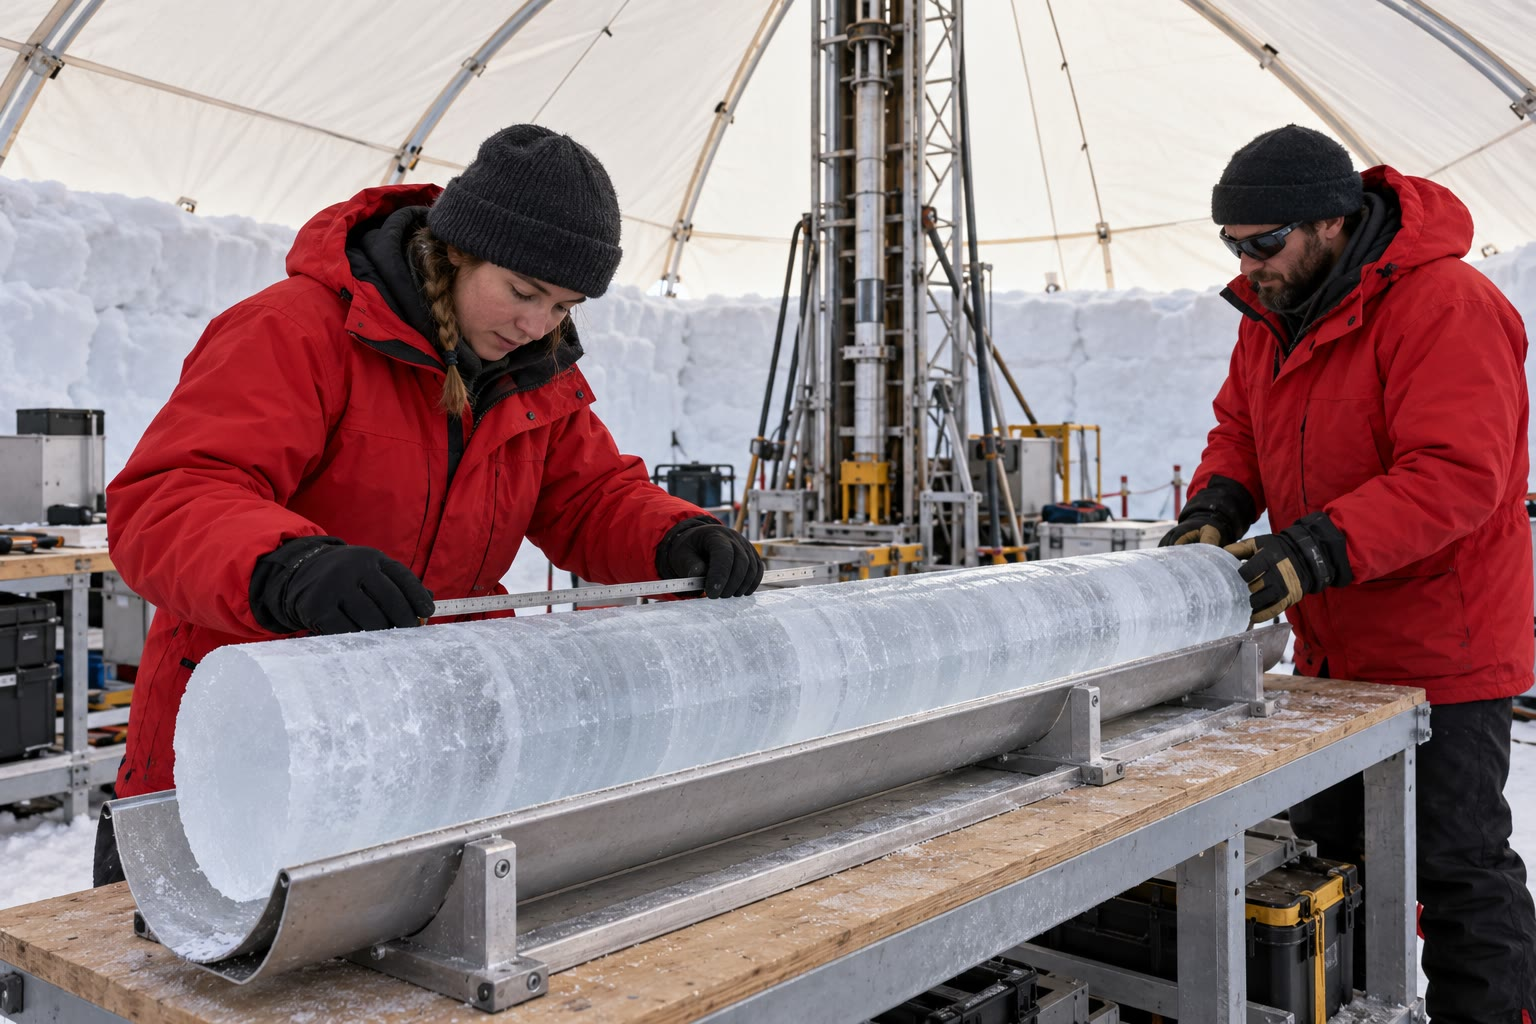
\includegraphics[width=\linewidth]{images/book5/ai/b3-ice-core-tent.jpg}

{\scriptsize 在冰盖上钻探帐篷内的托架中测量冰芯，
后方为钻塔（AI 生成示意图）。}
\end{minipage}
\end{inthelab}

\section{练习}

\begin{exercise}[$\star$]\label{exo:b3:stable-isotopes:1}
一方解石的 $\delta^{18}\mathrm O = \qty{30.5}{\permil}$，其生长所用的水为
\qty{-2.1}{\permil}，两者均以 VSMOW 为标准。计算 $\alpha$、$1000\ln\alpha$ 与
$\Delta$。后两者相差多少？
\end{exercise}

\begin{exercise}[$\star$]\label{exo:b3:stable-isotopes:2}
某高纬度沿海台站的年平均气温为
\qty{-25}{\celsius}。利用本章针对此类台站的关系式，
预测其降水的
$\delta^{18}\mathrm O$、$\delta\mathrm D$ 与\omterm{def:b3:stable-isotopes:d-excess}{氘盈余}。
\end{exercise}
% ledger: dansgaard64:effects

\begin{exercise}[$\star$]\label{exo:b3:stable-isotopes:3}
某盆地中碳酸盐的 $\delta^{13}\mathrm C = \qty{+1.0}{\permil}$，有机质的
为 \qty{-26.0}{\permil}。输入端取 \qty{-5}{\permil}，计算
$f_{\mathrm{org}}$。
\end{exercise}
% ledger: planavsky22:forg

\begin{exercise}[$\star$]\label{exo:b3:stable-isotopes:4}
某腕足壳的 $\Delta_{47} = \qty{0.600}{\permil}$。利用
本章的标定关系，求其生长时的温度。
\end{exercise}
% ledger: isogeochem:d47

\begin{exercise}[$\star\star$]\label{exo:b3:stable-isotopes:5}
水汽自海洋逸出时 $\delta^{18}\mathrm O = \qty{-13}{\permil}$，并
以恒定的 $\alpha = 1.0100$ 持续降水。当水汽达到
\qty{-33}{\permil} 时，剩余水汽的比例为多少？此时
降水的 $\delta^{18}\mathrm O$ 为多少？
\end{exercise}
% ledger: white13c9:rayleigh

\begin{exercise}[$\star\star$]\label{exo:b3:stable-isotopes:6}
雪样为 \qty{-40}{\permil}，与 \qty{0}{\permil} 的海水相比较。计算 $\alpha$、
$1000\ln\alpha$、$1000(\alpha - 1)$ 以及两者之间的 $\Delta$。
命题中的哪一项近似失效？失效程度为多少？
\end{exercise}

\begin{exercise}[$\star\star$]\label{exo:b3:stable-isotopes:7}
某有孔虫的 $\delta^{18}\mathrm O = \qty{+1.50}{\permil}$（VPDB 标准），其生长于
\qty{0.00}{\permil}（VSMOW 标准）的水中。用本章的方法计算其生长温度，
并说明水的
\qty{0.1}{\permil} 的误差会使温度改变多少。
\end{exercise}
% ledger: isogeochem:ko97

\begin{exercise}[$\star\star$]\label{exo:b3:stable-isotopes:8}
底栖叠层曲线自现在至末次盛冰期变化了 \qty{1.77}{\permil}。
扣除本章计算的冰量份额，并利用
\qty{2}{\celsius} 附近方解石标定曲线的斜率，
将其余部分换算为深层水温的变化。
\end{exercise}
% ledger: data:lr04, white13c9:ice-volume, isogeochem:ko97

\begin{exercise}[$\star\star$]\label{exo:b3:stable-isotopes:9}
某黄铁矿的 $\delta^{34}\mathrm S = \qty{10.0}{\permil}$，且 $\delta^{33}\mathrm S =
\qty{8.2}{\permil}$。计算 $\Delta^{33}\mathrm S$。这一结果说明了
黄铁矿形成时大气的什么状况？
\end{exercise}
% ledger: white13c9:s-mif

\begin{exercise}[$\star\star\star$]\label{exo:b3:stable-isotopes:10}
在封闭系统凝结中，水汽与生成的全部凝结物始终
保持平衡共存。证明此时水汽满足 $R_v/R_{v,0} = 1/[f +
\alpha(1 - f)]$，并将其与\omterm{prop:b3:stable-isotopes:rayleigh-distillation}{瑞利蒸馏}相比较，
取 $f = 0.2$ 与 $\alpha = 1.01$。
\end{exercise}

\begin{exercise}[$\star\star\star$]\label{exo:b3:stable-isotopes:11}
由估计可知，\qty{2000}{Gt} 甲烷碳的
同位素组成为 \qty{-60}{\permil}，使可交换碳偏移了 \qty{-2.5}{\permil}，
在 $\delta_0 = 0$ 的条件下，求由此隐含的储库质量。以该质量计，
\qty{-25}{\permil} 的有机碳需要多少，才能产生相同的偏移？
与已发表的取值范围相比较。
\end{exercise}
% ledger: dickens11:petm

\begin{exercise}[$\star\star\star$]\label{exo:b3:stable-isotopes:12}
证明：沿降温路径，$\mathrm d\delta_v/\mathrm dT = (\alpha - 1)(1000 +
\delta_v)\,\mathrm d\ln e_s/\mathrm dT$。在 \qty{-20}{\celsius} 时，本章模型中的水汽
$\delta^{18}\mathrm O = \qty{-49.1}{\permil}$，
升华曲线给出 $\mathrm d\ln e_s/\mathrm dT =
\qty{0.0960}{K^{-1}}$，计算此处的斜率。
\end{exercise}
% ledger: gkinis14:alpha-ice, iapws:melt-subl

\section{问题：一滴雨的旅程，前往伊尔斯冰穹}

\begin{problem}[{周末问题——沿虚构冰盖考察路线的雪同位素、
古温度与碳偏移}]\label{pb:b3:stable-isotopes:1}
一气团以 \qty{0}{\celsius} 离开虚构冰盖的边缘，其水汽的
$\delta^{18}\mathrm O = \qty{-20.0}{\permil}$ 与 $\delta\mathrm D =
\qty{-150}{\permil}$，并在恒压下随其向内陆运动而降温。
雪于海岸站 \qty{-10}{\celsius} 时形成，于中途站 \qty{-20}{\celsius} 时形成，
于伊尔斯冰穹 \qty{-30}{\celsius} 时形成，此时剩余水汽的比例
分别为 $f = 0.425$、$0.169$ 与 $0.0622$。采用本章的冰–汽
分馏系数，各段内取其中点温度处的值，
并在该段内保持不变。
% ledger: gkinis14:alpha-ice, iapws:melt-subl, dansgaard64:effects, isogeochem:ko97, isogeochem:d47, white13c9:ice-volume, data:lr04, planavsky22:forg, dickens11:petm

\medskip\noindent\textbf{第一部分——蒸馏。}
\begin{enumerate}
\item 计算 $\alpha^{18}$ 与 $\alpha^{\mathrm D}$ 在 $-5$、$-10$、$-15$、$-20$、
$-25$ 与 \qty{-30}{\celsius} 时的值（氧取五位有效数字，
氘取四位）。
\item 计算水汽到达海岸站时的 $\delta^{18}\mathrm O$。
\item 计算海岸站雪的该值。
\item 对中途站重复上述计算（$f$ 的段间比值为 $0.169/0.425$）。
\item 对伊尔斯冰穹重复上述计算。
\item 伊尔斯冰穹处，水汽原有的氧-18 中
仍留在空气中的比例为多少？
\end{enumerate}

\medskip\noindent\textbf{第二部分——温度与氘。}
\begin{enumerate}[resume]
\item 计算雪的 $\delta^{18}\mathrm O$ 随凝聚温度的斜率，
范围从海岸到伊尔斯冰穹。
\item 格陵兰各站的关系式会将伊尔斯冰穹的雪
对应到哪一个年平均地表温度？为何它可能与
\qty{-30}{\celsius} 不同？
\item 用同样的方法计算三个站点雪的 $\delta\mathrm D$。
\item 计算它们的\omterm{def:b3:stable-isotopes:d-excess}{氘盈余}。它在内陆如何变化？
\item 伊尔斯冰穹的雪是否位于大气降水线上？模型遗漏了
真实雪形成过程中包含的哪些因素？
\end{enumerate}

\medskip\noindent\textbf{第三部分——海岸外的一种有孔虫。} 海岸外取得的一根沉积岩芯
给出底栖有孔虫的 δ 值：顶部为 \qty{3.25}{\permil}
（VPDB），末次盛冰期为 \qty{5.02}{\permil}；底层水
今天相对于 VSMOW 为 \qty{0.00}{\permil}。
\begin{enumerate}[resume]
\item 计算当前底层水的温度，
采用方解石校准式。
\item 假设水的组成不变，计算冰期温度。这一
结果是否可能？
\item 对冰期底层水作修正，考虑 \qty{125}{m} 的海平面下降，
并重新计算。冰期底层水的降温幅度为多少？
\item 计算两个温度下预期的 $\Delta_{47}$，
以及它们的差值。
\item 为什么\omterm{def:b3:stable-isotopes:clumped}{团簇同位素}温度计不需要
水的组成？
\end{enumerate}

\medskip\noindent\textbf{第四部分——一次碳漂移。} 在岩芯更深处，
碳酸盐的 δ 值为 \qty{+0.5}{\permil}，中间被
一次短暂的 \qty{-3.0}{\permil} 漂移打断。
\begin{enumerate}[resume]
\item 漂移之前，取 $\delta_{\mathrm{in}} = \qty{-5}{\permil}$ 与
$\Delta_B = \qty{-28}{\permil}$，计算 $f_{\mathrm{org}}$。
\item 取练习 11 中的储库，0 时刻为 \qty{46000}{Gt}。
若来源是 \qty{-60}{\permil} 的甲烷，漂移需要多少碳？
\item 若来源是 \qty{-25}{\permil} 的有机碳，又需要多少碳？
\item 若来源是 \qty{-5}{\permil} 的地幔碳，又需要多少碳？
\item 同一岩芯中的哪一项观测有助于
在这些来源之间作出判断？
\item 说明伊尔斯冰穹降落的雪的 $\delta^{18}\mathrm O$。
\end{enumerate}
\end{problem}
